% Lecture Template for ME3001-001-Tristan Hill - Spring 2017 - Fall 2017
% 
% Mechanical Engineering Analysis with MATLAB
%
% Roots of Non- Linear Equations

% Document settings
\documentclass[11pt]{article}
\usepackage[margin=1in]{geometry}
\usepackage[pdftex]{graphicx}
\usepackage{multirow}
\usepackage{setspace}
\usepackage{hyperref}
\usepackage{color,soul}
\usepackage{fancyvrb}
\usepackage{framed}
\usepackage{wasysym}
\usepackage{multicol}

\pagestyle{plain}
\setlength\parindent{0pt}
\hypersetup{
    bookmarks=true,         % show bookmarks bar?
    unicode=false,          % non-Latin characters in Acrobat’s bookmarks
    pdftoolbar=true,        % show Acrobat’s toolbar?
    pdfmenubar=true,        % show Acrobat’s menu?
    pdffitwindow=false,     % window fit to page when opened
    pdfstartview={FitH},    % fits the width of the page to the window
    pdftitle={My title},    % title
    pdfauthor={Author},     % author
    pdfsubject={Subject},   % subject of the document
    pdfcreator={Creator},   % creator of the document
    pdfproducer={Producer}, % producer of the document
    pdfkeywords={keyword1} {key2} {key3}, % list of keywords
    pdfnewwindow=true,      % links in new window
    colorlinks=true,       % false: boxed links; true: colored links
    linkcolor=red,          % color of internal links (change box color with linkbordercolor)
    citecolor=green,        % color of links to bibliography
    filecolor=magenta,      % color of file links
    urlcolor=blue           % color of external links
}

% assignment number 
\newcommand{\NUM}{1 } 
\newcommand{\VSpaceSize}{2mm} 
\newcommand{\HSpaceSize}{2mm} 

\definecolor{mygray}{rgb}{.6, .6, .6}

\setulcolor{red} 
\setstcolor{green} 
\sethlcolor{mygray} 

\begin{document}

\textbf{ \LARGE ME 3001 Lecture - Roots of Non-Linear Equations} \\

\begin{itemize}


	\item \textbf{ \LARGE What is a Non-Linear Equation ? }
			
			\Large{" an equation whose graph does not form a straight line"} \\ \vspace{20mm}


	\item \textbf{ \LARGE Different Types of Non-Linear Equations }
		
		\begin{itemize}
			\item \textbf{\Large Polynomials (excluding first order)} \vspace{30mm}
			\item \textbf{\Large Transcendentals} \vspace{10mm}

\Large{" a transcendental function "transcends" algebra in that it cannot be expressed in terms of a finite sequence of the algebraic operations of addition, multiplication, and root extraction. Examples of transcendental functions include the exponential function, the logarithm, and the trigonometric functions. "}\\
				\begin{itemize}
					\item Exponentials \vspace{10mm}
					\item Logarithms \vspace{10mm}
					\item Trigonometrics \vspace{5mm}
				\end{itemize}

		\end{itemize}

	\item \textbf{ \LARGE What does "Solve the Equation" mean?}
	\newpage

	\item \textbf{ \LARGE Let us do a simple example} \\\\
	
		\hspace{20mm}\scalebox{1.5}{$y = x^2 + 2x - 10$}	 \vspace{80mm}
		
		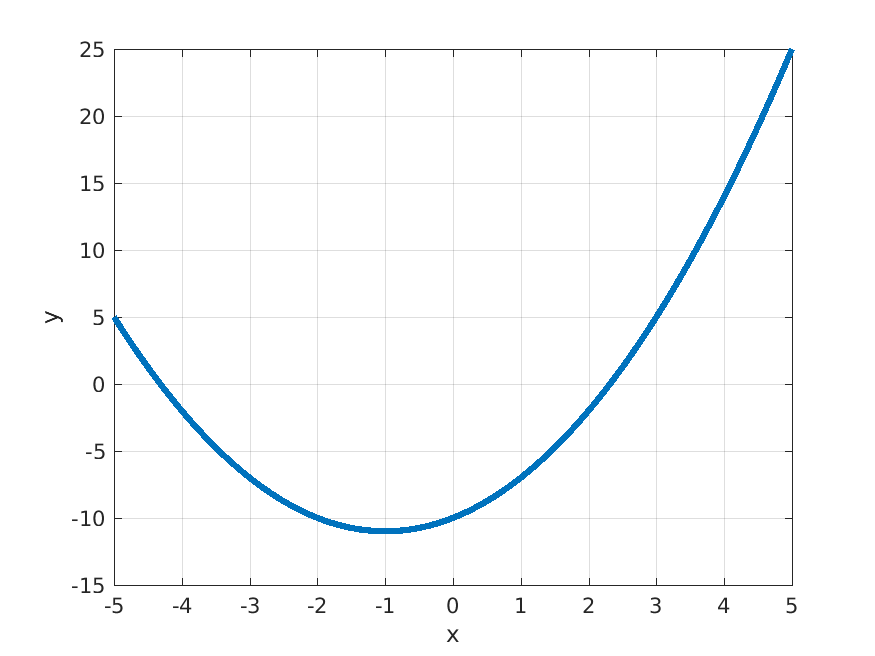
\includegraphics[scale=1]{lecture1_fig1.png}
		
		\newpage


	\item \textbf{ \LARGE Method 1 - {\it The Incremental Search} }

		

			\begin{itemize}
			\item \Large{ We are looking for where the line crosses the x-axis, so how can we tell if this happens?} \\ 
			\item \Large{ Let us investigate with our simple example.} \\ 

			 \hspace{20mm}\scalebox{1.5}{$y = x^2 + 2x - 10$}\vspace{20mm}\\
		\end{itemize}
			
\includegraphics[scale=.3]{lecture1_fig4.png}
			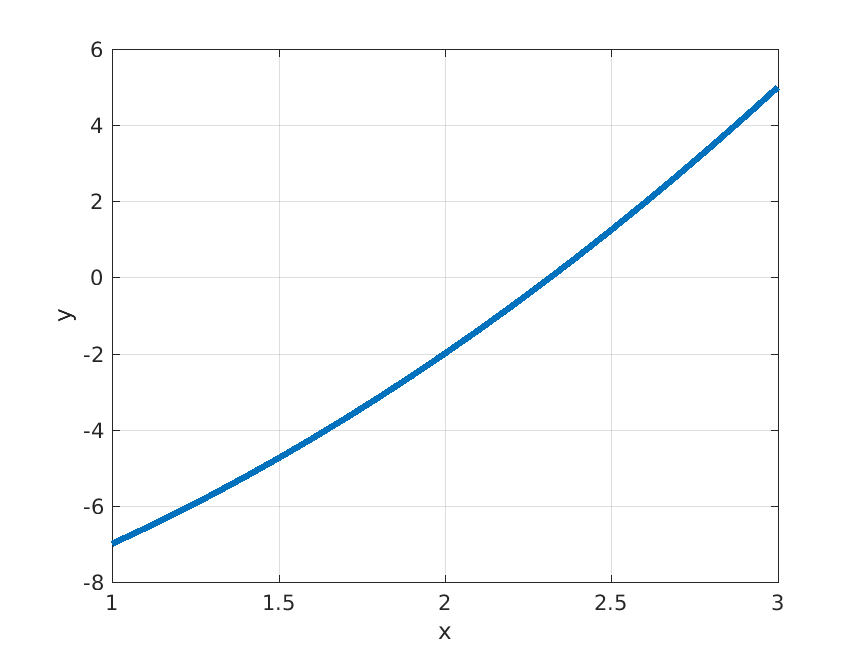
\includegraphics[scale=.8]{lecture1_fig3.png}

		\newpage
		\item \textbf{ \LARGE Method 2 - {\it The Bisection Method} } \\
			\begin{itemize}
				\item different than the previous method because it is a {\it bracketing method}\\
				\item It is a faster method in general but can you think of any tradeoffs?\\ \vspace{20mm}
			\end{itemize}
	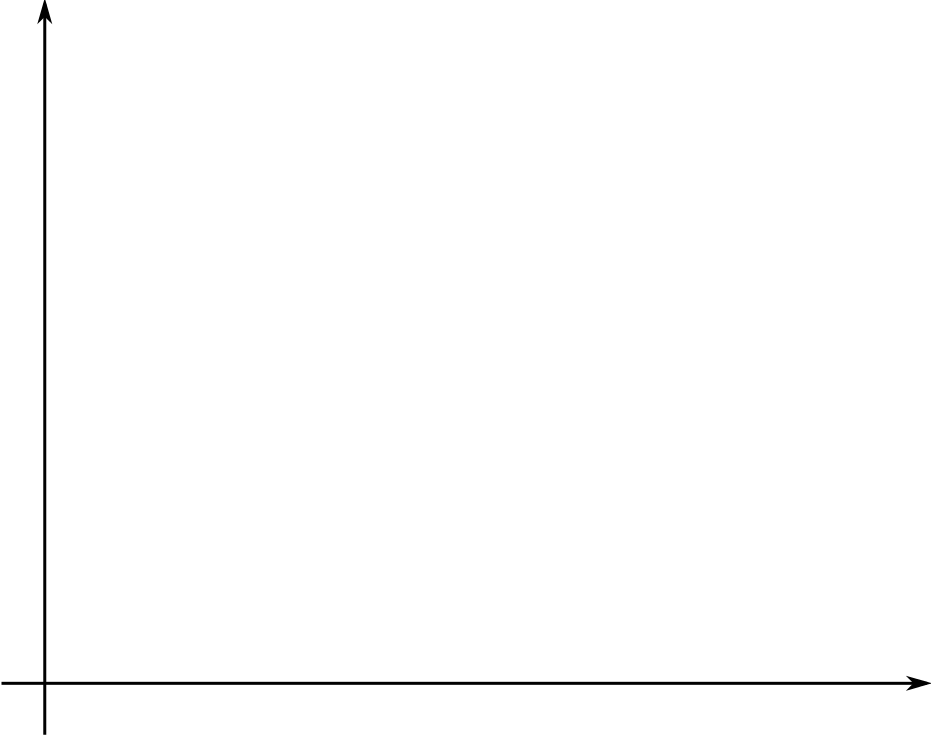
\includegraphics[scale=.5]{lecture1_fig5.png}

	\newpage
	\item \textbf{ \LARGE {\it Advantages, Disadvantages, and Pitfalls} } \\\\
	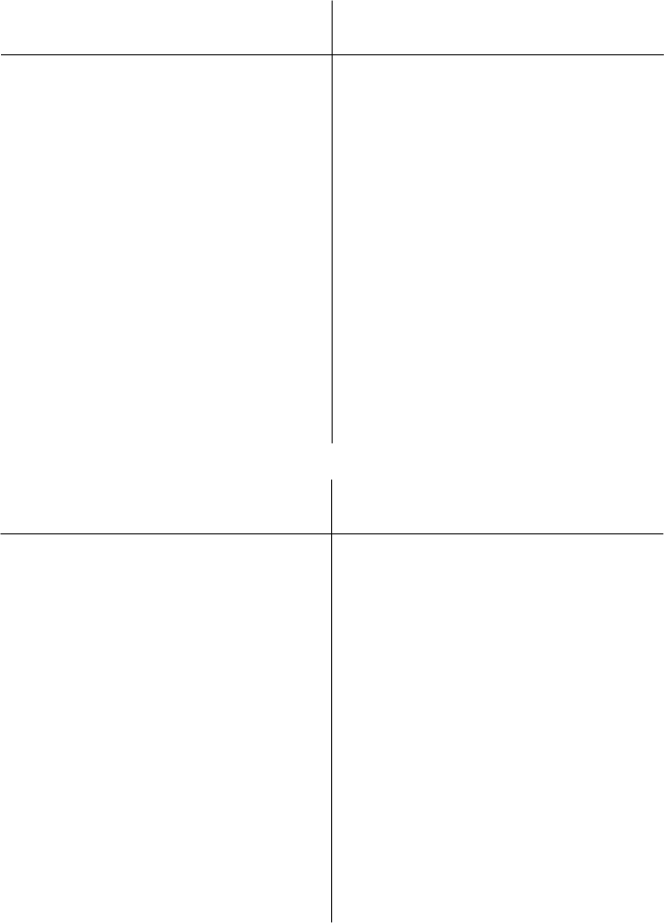
\includegraphics[scale=.65]{lecture1_fig6.png}
\newpage

	\item \textbf{ \LARGE It is useful to have generalized methods }\\
		\begin{itemize}
			\item \Large{A solution technique for the general problem}\\		
			\item \Large{Standard set of steps or {\it algorithm} for finding the solution}\\\\
		\end{itemize}

	\item \textbf{ \LARGE The general {\it root-finding} problem }\\\\\\
	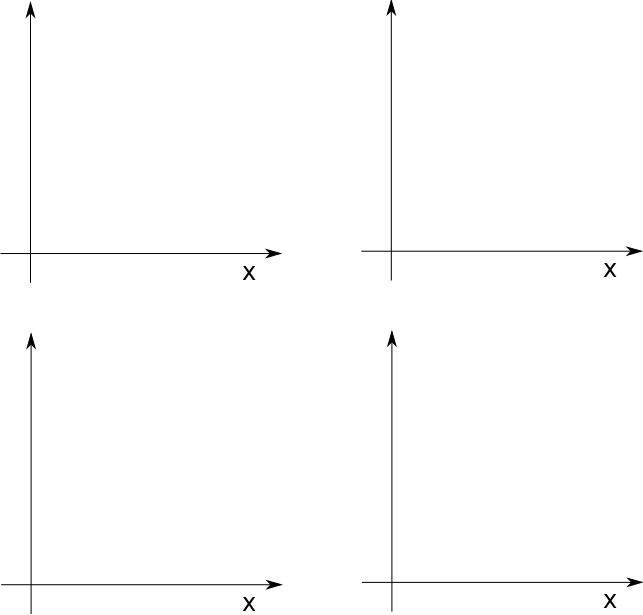
\includegraphics[scale=.6]{lecture1_fig2.png}
	\newpage 

	\item \textbf{ \LARGE REMINDER - Homework 1 is posted on ilearn } \\
	
	 \textbf{ \LARGE DUE: Wednesday, Sep. 5}	\\\\

	\item \textbf{ \LARGE REMINDER - Instructions for Installing MATLAB on your computer have been posted on ilearn. } \\
	

\end{itemize}


	

\end{document}



